\section{Seberapa kuat hasilnya?}\label{sec:diagnostics}
\subsection{Tidak cukup hanya melihat p-value}
Dari 176 model utama, 95 memenuhi keputusan F dan t bounds pada 5\%. Setelah pemeriksaan long run tambahan, jumlahnya menjadi 62. Sebanyak 28 juga lolos diagnostic tests yang dipakai.

Angka 28 tidak berarti hanya 28 model yang benar. Ini hasil dari satu kumpulan aturan pemeriksaan. Kita tetap perlu melihat tes mana yang memberi catatan dan apa artinya bagi kesimpulan.

Diagnostic tests memeriksa residual, yaitu selisih data aktual dengan nilai yang diperkirakan model. Beberapa istilahnya:
\begin{itemize}
\item \textbf{Autocorrelation}: residual masih berkaitan antarperiode.
\item \textbf{Heteroskedasticity dan ARCH}: variasi residual tidak selalu tetap.
\item \textbf{RESET}: ada indikasi bentuk model perlu ditinjau.
\item \textbf{Normality test}: distribusi residual berbeda dari distribusi normal yang diuji.
\item \textbf{CUSUM dan CUSUMSQ}: membantu memeriksa stabilitas sepanjang waktu.
\end{itemize}

Masalah-masalah ini tidak sama. Residual yang tidak normal, misalnya, tidak otomatis berarti OLS tidak konsisten. Menggabungkan semua tes menjadi satu status bersih merupakan pilihan yang cukup hati-hati.

Tes yang tidak menemukan masalah juga belum membuktikan model pasti benar. Sampel kecil bisa membuat tes kurang kuat. Diagnostic tests pun belum menyelesaikan masalah sebab-akibat atau variabel penting yang belum masuk.

\subsection{Bagaimana stabilitas diperiksa?}
CUSUM utama diambil dari Stata \cite{stata}. Nilai jalurnya cocok dengan statistik tersimpan untuk seluruh 176 model utama. Perhitungan independen juga cocok ketika data awal memungkinkan semua parameter dibedakan dengan baik.

Dua pengecualian adalah modal dan konsumsi Australia pada NARDL. Data awalnya belum cukup untuk membedakan semua parameter, atau belum \emph{full rank}. Perhitungan independen menunggu sampai kondisi tersebut terpenuhi, sehingga cara memulainya berbeda dari Stata. Hasil resmi Stata tetap dipakai dan model diberi catatan. Ini berbeda dari model total bilateral Australia.

CUSUMSQ memakai pendekatan Monte Carlo dengan 19.999 simulasi dan seed tetap. Batas pembanding dihitung melalui simulasi yang bisa diulang. Simulasi ini memakai acuan distribusi normal. Hasilnya masih pendekatan, bukan salinan persis tabel paper acuan.

\begin{figure}[!htbp]\centering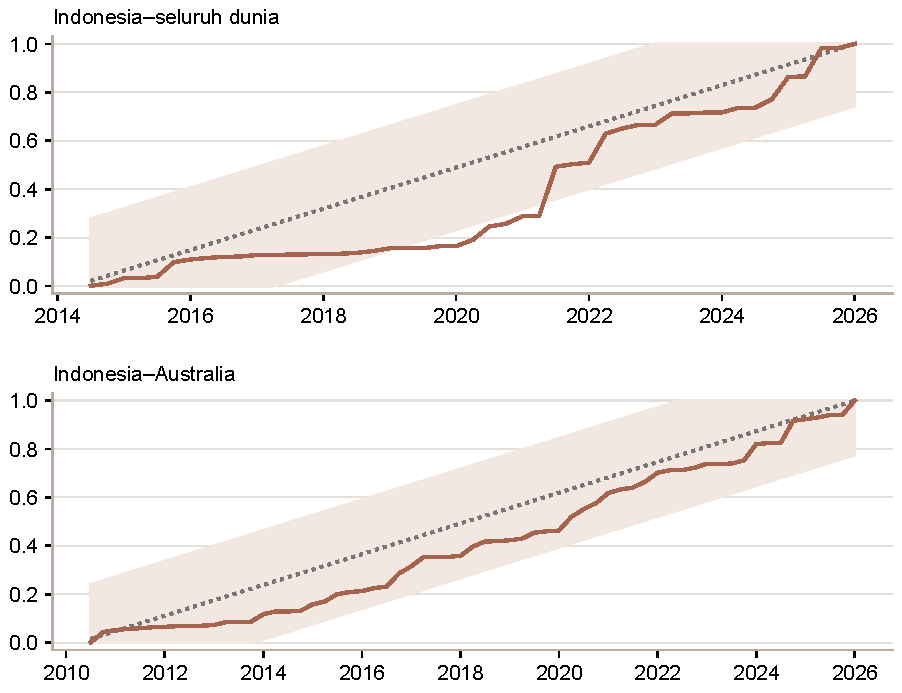
\includegraphics[width=\linewidth]{assets/stability.pdf}
\caption{CUSUMSQ total Indonesia dan Indonesia--Australia. Grafik ini memeriksa stabilitas residual; area berwarna bukan confidence interval efek kurs.}\label{fig:stability}
\end{figure}

Pada total Indonesia, CUSUMSQ memberi catatan stabilitas. Pada Australia, pemeriksaan utama tidak menemukan masalah itu. Perhitungan model juga sudah dicocokkan antara persamaan level dan error correction serta dengan fitted values OLS independen. Cek numerik lulus, tetapi itu belum membuktikan semua asumsi ekonomi benar.

\subsection{Apa itu robustness check?}
Robustness check melihat apakah hasil berubah saat pilihan analisis diubah. Run ini mencoba maksimum lag yang lebih pendek, menambah BCOM, memperpanjang data total ke 2006, memakai WPI India, dan memakai keluarga kurs GEM untuk beberapa mitra.

Arah negatif komoditas total dan energi/tambang bertahan pada beberapa ARDL pembanding. Tetapi sebagian mendapat catatan diagnostic tests. Pada NARDL, koefisien depresiasinya belum signifikan dan status long run dapat berubah menurut lag.

\begin{table}[!htbp]\centering\caption{Robustness checks ARDL komoditas Indonesia}
{\small\setlength{\tabcolsep}{3pt}\renewcommand{\arraystretch}{1.15}
\begin{tabular}{p{0.08\linewidth}p{0.2\linewidth}p{0.08\linewidth}p{0.2\linewidth}p{0.15\linewidth}p{0.12\linewidth}}
\toprule
\textbf{Kel.} & \textbf{Varian} & \textbf{N} & \textbf{Koef. kurs} & \textbf{p} & \textbf{Status}\\
\midrule
G6 & Utama & 61 & -1,355 & \(<0{,}001\) & L+D\\
G6 & Cap 2 & 63 & -1,536 & \(<0{,}001\) & L+D\\
G6 & BCOM & 61 & -1,378 & \(<0{,}001\) & L\\
G7 & Utama & 61 & -2,040 & \(<0{,}001\) & L+D\\
G7 & Cap 2 & 63 & -2,222 & \(<0{,}001\) & L\\
G7 & BCOM & 61 & -2,305 & \(<0{,}001\) & L\\
\bottomrule
\end{tabular}
}\label{tab:sens}
\end{table}

BCOM adalah indeks harga luas. Ia bisa bergerak bersama permintaan global, energi, dan kondisi keuangan. Menambahkannya membantu memeriksa perubahan hasil, tetapi belum membuktikan bahwa harga global adalah penyebab yang sudah berhasil dipisahkan.

Perubahan sumber bisa mengubah konsep dan periode data sekaligus. Jadi, tidak semua robustness check hanya mengubah satu hal pada sampel identik.

Tiga NARDL India dengan BCOM tidak mempunyai hasil bounds finite-sample yang tersedia: komoditas total, energi/tambang, dan bahan baku/penolong. Ketiganya memakai 49 observasi dan 25--27 parameter. Koefisien tetap tersedia; uji yang tidak tersedia tidak diubah menjadi keputusan lolos atau gagal.

\subsection{Mengapa pola J berkurang setelah diperiksa?}
Aturan membaca garis utama di PPT dan paper adalah
\begin{equation}
 \min_{0\le h\le4}R_h^{J,-}<0,\qquad
 \frac{1}{9}\sum_{h=16}^{24}R_h^{J,-}>0.\label{eq:jvisual}
\end{equation}
Artinya, ada setidaknya satu bagian negatif pada tahun pertama dan rata-rata bagian akhir positif. Ini aturan untuk membantu pelaporan, bukan uji J-curve formal paper. Aturan tersebut juga tidak ditetapkan sebelum hasil penelitian dilihat.

\begin{table}[!htbp]\centering\caption{Pola J sebelum dan sesudah pemeriksaan tambahan}
{\small\setlength{\tabcolsep}{3pt}\renewcommand{\arraystretch}{1.15}
\begin{tabular}{p{0.18\linewidth}p{0.12\linewidth}p{0.15\linewidth}p{0.21\linewidth}p{0.23\linewidth}}
\toprule
\textbf{Model} & \textbf{Seri} & \textbf{J titik} & \textbf{J + L+D} & \textbf{Dua fase CI}\\
\midrule
ARDL & 88 & 10 & 1 & 0\\
NARDL & 88 & 24 & 5 & 2\\
\bottomrule
\end{tabular}
}\label{tab:j}
\end{table}

Ada sepuluh pola J pada garis utama ARDL dan 24 pada NARDL. Setelah cek long run dan diagnostic tests, tersisa satu ARDL dan lima NARDL. Jika fase awal dan akhir juga harus terpisah dari nol pada confidence interval yang digunakan, tersisa nol ARDL dan dua NARDL.

Dua NARDL itu adalah modal Korea dan konsumsi AS. Masih ada proses mencari salah satu horizon awal, sehingga hasil ini belum menjadi satu uji simultan semua fase. Kelompok yang tumpang tindih juga membuat jumlah kasus tidak bisa dibaca sebagai frekuensi J-curve pada seluruh perdagangan.

\subsection{Mengapa ARDL dan NARDL bisa berbeda?}
NARDL menambah parameter dan membagi perubahan kurs menjadi dua seri. Seri tersebut juga bisa bergerak bersama aktivitas ekonomi. Pada data terbatas, angka untuk satu arah kurs dapat menjadi lebih tidak pasti.

AIC juga dapat memilih lag berbeda. ARDL yang lebih sederhana bisa lebih presisi, tetapi batasan simetrinya mungkin terlalu kuat. Perbedaan hasil belum otomatis membuktikan salah satunya paling benar.

Karena itu, model tidak dipilih hanya dari tanda yang sesuai hipotesis. Ketidaksepakatan hasil linier dan nonlinear perlu ikut dijelaskan sebagai temuan.
